% !TeX root = ../main.tex

\chapter{基于模型集成的样本筛选算法}

\section{条件风险价值CVaR}

虽然目前最先进的基于模型的方法已经取得了显著的性能,但它们通常只适合于训练的环境,当部署到扰动的真实环境时,性能往往会急剧下降。条件风险价值(CVaR)是一种用于计算最大风险的指标,借由CVaR指标,我们可以通过学习消极样本数据来提高强化学习算法的鲁棒性,得以解决强化学习算法中安全性不足的一大挑战。

\begin{figure}
  \centering
  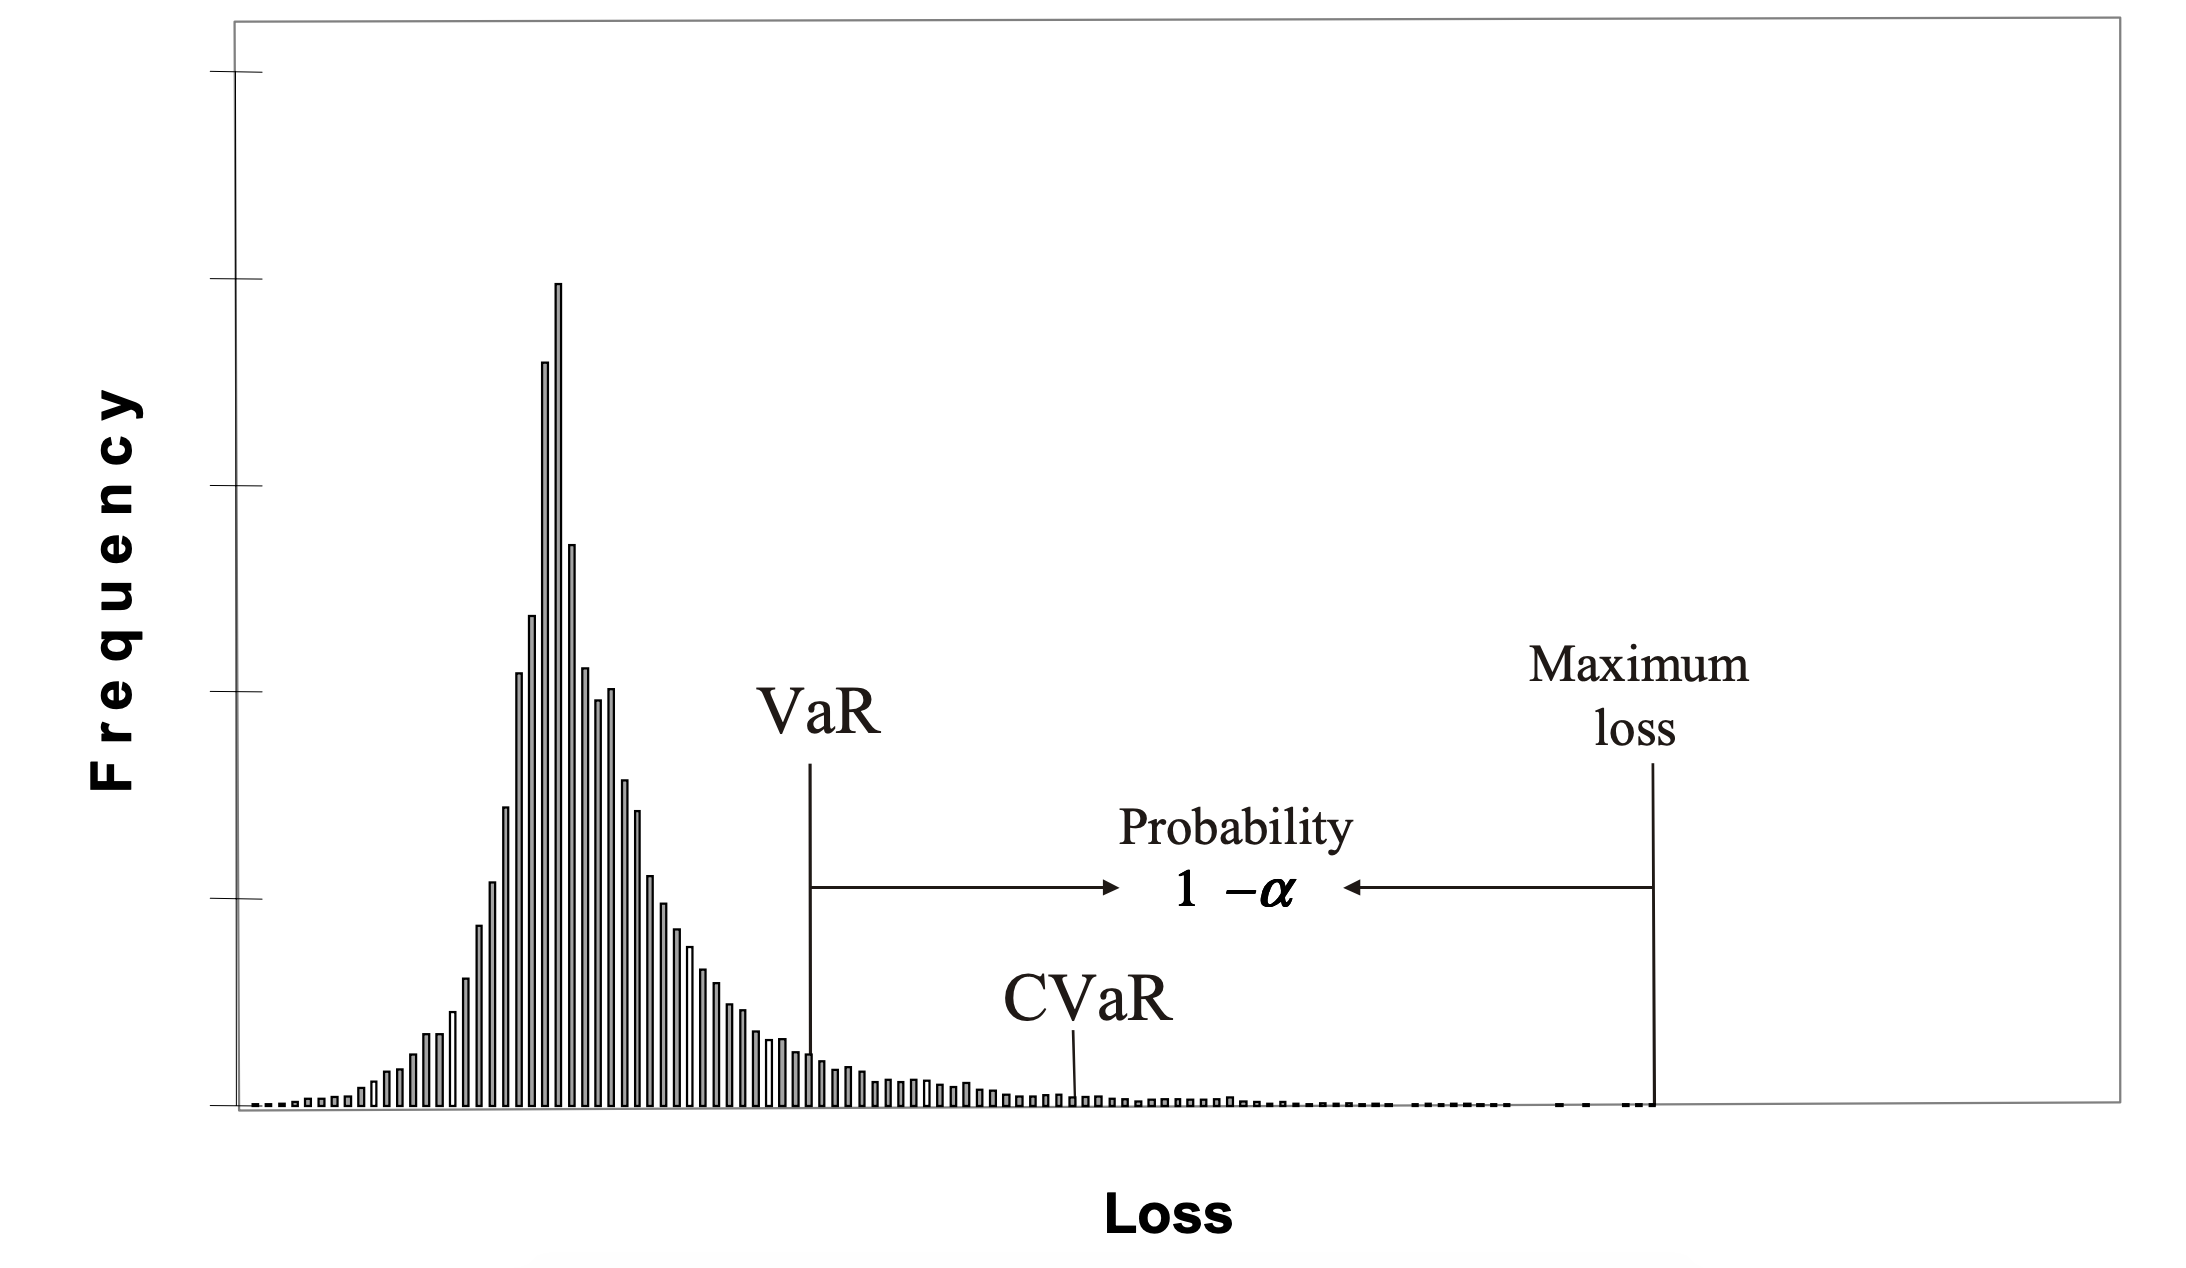
\includegraphics[width=\linewidth]{figures/CVaR.png}
  \caption*{国外的期刊习惯将图表的标题和说明文字写成一段,需要改写为标题只含图表的名称,其他说明文字以注释方式写在图表下方,或者写在正文中。}
  \caption{示例图片标题}
  \label{fig:cvar}
\end{figure}

如图\ref{fig:cvar}所示,首先定义风险价值(VaR):
\begin{equation}
    \mathrm{VaR}_\alpha=\inf\left\{z\mid\mathrm{P}(Z\geq z)\leq 1-\alpha\right\}
\end{equation}
VaR的含义为在给定置信度$\alpha$下的最大可能损失,更进一步地,我们可定义条件风险价值(CVaR):
\begin{equation}
    \mathrm{CVaR}_\alpha = \mathbb{E}\left[Z\mid Z\geq \mathrm{VaR}_\alpha\right]
\end{equation}
CVaR的含义为收益风险超过VaR部分的平均期望损失。

基于CVaR的思想,我们可以类似的在强化学习经验回放样本池中加入这一设计,将更低奖励反馈的样本加以更多的学习,而对过高奖励反馈的样本进行适当的筛选和丢弃,确保强化学习算法所学策略能够更稳定地处理高风险状态。但是这样的思路下尽管实现了鲁棒性的提升,但是显然易见的是筛选丢弃样本的做法会损失一部分性能。为此,我们提出了基于模型集成的强化学习样本筛选算法,在做到提升算法鲁棒性的同时维持原有的算法性能。

\section{环境模型的集成学习与筛选}\label{sec:model-method}

传统的不确定性环境建模和集成方法,虽然已经能够较好地模拟真实复杂环境并且捕捉到环境的不确定性 \cite{duan2007multi},但并不能很好地控制模拟的精准程度,本论文在不确定性环境建模的基础上,结合传统集成学习的方法,设计了模型的集成和筛选机制。

具体地,首先训练学习一组环境模型集合$\{\mathcal{M}_{\phi_1},\mathcal{M}_{\phi_2},\ldots\}$,集合中每一个环境模型都是一个概率神经网络,其输出$\mu_{\phi_i},\sigma_{\phi_i}$构成高斯分布$\mathcal{N}(\mu_{\phi_i}(s,a),\sigma_{\phi_i}(s,a))$,环境模型对于下一时刻的状态预测则服从该分布,即

\begin{equation}
    s^\prime \sim \mathcal{M}_{\phi_i}(s,a) = \mathcal{N}(\mu_{\phi_i}(s,a),\sigma_{\phi_i}(s,a))
\end{equation}

在训练环境模型的同时,根据真实环境中采样得到的真实样本$(S,A)$,可以计算并记录模型的期望偏差:
\begin{equation}
    \mathrm{bias}(\phi_i) = \underset{S,A\sim \pi,\mathcal{P}}{\mathbb{E}}\|\mathcal{M}_{\phi_i}(S,A)-\mathcal{P}(S,A)\|
\end{equation}

其中$\|\cdot\|$是状态空间$\mathcal{S}$上的范数距离,该式的含义为所训练的环境模型$\mathcal{M}$与真实环境$\mathcal{P}$之间的范数意义距离。在上述模型集合的基础上,首先根据所计算的$\mathrm{bias}(\phi_i)$大小进行升序重排,并设定一个概率参数$\alpha\in(0,1]$,筛选出$\mathrm{bias}$在$\alpha$分位数以前的模型,保留得到筛选后的模型集合$\mathcal{M}^\alpha = \{\mathcal{M}_{\phi_1},\mathcal{M}_{\phi_2},\ldots,\mathcal{M}_{\phi_{N_\alpha}}\}$,其中$N_\alpha$是前面所描述的升序排序后的集合索引$\left\{1,2,\ldots,N_\alpha,\ldots\right\}$中的$\alpha$分位数。

需要注意的是,用于集成的不确定性模型集合并不是$\mathrm{bias}$越小越好,过小的$\mathrm{bias}$可能意味着过拟合的环境模型。参数$\alpha$的重要用处是可以动态地调整模型集合的整体精确性,它能与下一节将介绍的参数$\beta$协作调整强化学习的收益性能与鲁棒性。

\section{环境模型的数据生成与筛选}\label{sec:rollout-method}

传统的基于模型的强化学习算法在得到环境模型后,往往是以期望收益为目标进行最大化优化,但是期望意义下的最优并不意味着在任意环境下都能有优秀的表现,在实际部署策略的时候,当面临一些受干扰的信息不足的状态,策略容易做出一些不合理甚至危险的决策,导致强化学习在实际部署中不稳定。

为了解决这一问题,本论文提出了一种主动关注较坏情况的样本筛选机制,适当延缓强化学习训练速度,提升决策策略的鲁棒性。

具体地,基于上一节得到的$\mathcal{M}^{\alpha}$模型集合,在每一步都随机抽取一个模型$\mathcal{M}_{\phi_i}\in\mathcal{M}^\alpha$,然后使用该模型进行下一时刻的状态预测,即$s_{t+1}\sim \mathcal{M}_{\phi_t}(s_t,a_t), \phi_t\in\Phi_\alpha$,这样的一组状态和动作组成模拟样本$x=\left(s_{t+1},s_t,a_t\right)$,填入缓存池,然后相似地以一个概率参数$\beta\in(0,1]$进行筛选,从中挑选出反馈奖励值相对较低的样本,得到一个筛选后的$\beta$分位数样本集合

\begin{equation}
    \mathcal{B}_\beta^{\pi,\mathcal{M}^\alpha}=\left\{x|x\in\mathcal{B}^{\pi,\mathcal{M}^\alpha},r(x)\leq r_\beta(\mathcal{B}^{\pi,\mathcal{M}^\alpha})\right\}
\end{equation}
其中$\mathcal{B}^{\pi,\mathcal{M}^\alpha}=\left\{x|x\triangleq\left(s_{t+1},s_t,a_t\right)\sim\pi,\mathcal{M}^\alpha\right\}$, $r_\beta(\mathcal{B}^{\pi,\mathcal{M}^\alpha})$ 是缓存池 $\mathcal{B}^{\pi,\mathcal{M}^\alpha}$的$\beta$分位数。

缓存池里的模拟样本构成的期望收益记为${V}^{\pi,\mathcal{M}^\alpha}_\beta$。本论文可以证明,加入样本筛选机制后的模拟期望收益,与真实环境中期望收益的差异为一个受参数$\beta$控制的上界,如定理 \ref{the:beta-drop-bound} 所述。

\begin{theorem}\label{the:beta-drop-bound}

记$R_{m}$为奖励函数$r(s,a)$的上确界, 即 $R_{m}=\underset{s\in\mathcal{S},a\in\mathcal{A}}{\sup}r(s,a)$,在环境模型$\mathcal{M}_\phi$上使用样本筛选机制后,所得期望收益与真实环境中期望收益的差异值存在误差上界:

\begin{equation}
    |{V}_\alpha^{\pi, \mathcal{M}_{\phi}} - {V}^{\pi,\mathcal{M}_{\phi}}| \leq \frac{\alpha(1+\alpha)}{(1-\alpha)(1-\gamma)}\mathrm{R_{m}} \triangleq \epsilon_\alpha
\label{eq:eps-beta}
\end{equation}

\end{theorem}

定理~\ref{the:beta-drop-bound}的重要意义是,即使筛选掉一批模拟样本,环境模型给出的模拟数据仍具备一定的可靠性,该可靠性由概率参数$\alpha$控制。

为了证明上述定理,我们首先需要引入两个引理

\begin{lemma}\label{lem:proof-for-lem41}

定义

\begin{equation}\label{def:G-sa}
G^{\pi,\mathcal{M}}(s,a)=\underset{\hat{s}'\sim\mathcal{M}(\cdot|s,a)}{\mathbb{E}}{{V}^{\pi,\mathcal{M}}}(\hat{s}') - \underset{s'\sim\mathcal{P}(\cdot|s,a)}{\mathbb{E}}{{V}^{\pi,\mathcal{M}}}(s')
\end{equation}
对于任意策略 $\pi$ 和任意动态模型 $\mathcal{M},\mathcal{M}'$,存在如下关系式

\begin{equation}
{V}^{\pi,\mathcal{M}'} - {V}^{\pi,\mathcal{M}} = \frac{\gamma}{1-\gamma}\underset{S,A\sim\pi,\mathcal{M}}{\mathbb{E}}\left[G^{\pi,\mathcal{M}'}(S,A)\right]
\end{equation}

\end{lemma}

引理 \ref{lem:proof-for-lem41} 引用自Luo等人提出的定理,在其基础上,我们可以进一步推出如下的引理\ref{lem:mb-bound}。

\begin{lemma}\label{lem:mb-bound}
设基于模型方法所能取得的价值函数 ${V}^{\pi,\mathcal{M}}$ 在状态空间$\mathcal{S}$上是Lipschitz连续的,并设$K$为 Lipschitz常数,。记$\mathcal{P}$表示真实环境的状态转移概率分布,则有如下的不等式关系:
\begin{equation}
\left|{V}^{\pi, \mathcal{M}}-{V}^{\pi, \mathcal{P}}\right| \leq\frac{\gamma}{1-\gamma}K\cdot\mathrm{bias}
\end{equation}
其中
\begin{equation}
\mathrm{bias} \triangleq \underset{s,a\sim \pi,\mathcal{P}}{\mathbb{E}}\left\|\mathcal{M}(s, a)-\mathcal{P}(s, a)\right\|
\end{equation}

\label{theo:mb-bound}
\end{lemma}

在引理 \ref{lem:mb-bound}中, 我们假设了关于估计模型$\mathcal{M}$的期望收益${V}^{\pi,\mathcal{M}}(s)$ 是关于任意范数距离$\|\cdot\|$Lipschitz连续的,即
\begin{equation}\label{assum:lip}
    \left|{V}^{\pi,\mathcal{M}}(s)-{V}^{\pi,\mathcal{M}}(s^{\prime})\right| \leq K\left\|s-s^{\prime}\right\|, \forall s, s^{\prime} \in \mathcal{S}
\end{equation}
其中$K\in \mathbb{R}^+$ 是一个Lipschitz常数。该假设的意义是相近的状态应该拥有相似的价值估计,对于绝大多数场景而言,这一假设显然都是成立的。引理~\ref{lem:mb-bound}的证明如下:

\begin{proof}

根据$G^{\pi,\mathcal{M}}(s,a)$在公式(\ref{def:G-sa})的定义,以及假设(\ref{assum:lip})即 ${V}^{\pi,\mathcal{M}}(s)$ 满足 Lipschitz 连续性, 我们可以得到

\begin{equation}\label{eq:G-leq}
|G^{\pi,\mathcal{M}}(s,a)|\leq K\|\mathcal{M}(s,a)-\mathcal{P}(s,a)\|
\end{equation}
Then, we can show that

\begin{align*}
\left|{V}^{\pi, \mathcal{M}}-{V}^{\pi, \mathcal{P}}\right| &= \frac{\gamma}{1-\gamma}\left|\underset{s,a\sim\pi,\mathcal{P}}{\mathbb{E}}\left[G^{\pi,\mathcal{M}}(s,a)\right]\right| \tag{By Lemma \ref{lem:proof-for-lem41}}\\
&\leq \frac{\gamma}{1-\gamma}\underset{s,a\sim\pi,\mathcal{P}}{\mathbb{E}}\left[\left|G^{\pi,\mathcal{M}}(s,a)\right|\right] \tag{By Triangle Inequality}\\
&\leq \frac{\gamma}{1-\gamma}\underset{s,a\sim\pi,\mathcal{P}}{\mathbb{E}}K\|\mathcal{M}(s,a)-\mathcal{P}(s,a)\| \tag{By equation (\ref{eq:G-leq})}\\
&= \frac{\gamma}{1-\gamma}K\cdot\underset{s,a\sim\pi,\mathcal{P}}{\mathbb{E}}\|\mathcal{M}(s,a)-\mathcal{P}(s,a)\|\\
&\triangleq \frac{\gamma}{1-\gamma}K\cdot\mathrm{bias}
\end{align*}

\end{proof}

基于引理~\ref{lem:mb-bound},我们可以证明定理~\ref{the:beta-drop-bound}。



% 更进一步,将\ref{sec:model-method}中的模型筛选机制加入进来,本论文已经证明,在这两个筛选机制的共同作用下,模型给出的模拟数据依然是可靠并且可控的,如定理\ref{the:MBDP-bound}所述。

% \begin{theorem}\label{the:MBDP-bound}

% 加入模型筛选机制和样本筛选机制后的模拟期望收益${V}_\beta^{\pi, \mathcal{M}^\alpha}$与真实环境$\mathcal{P}$中的期望收益${V}^{\pi, \mathcal{P}}$的差异值存在误差上界:

% \begin{equation}
% \left|{V}_\beta^{\pi, \mathcal{M}^\alpha}-{V}^{\pi, \mathcal{P}}\right|\leq D_{\alpha,\beta}(\mathcal{M})
% \end{equation}
% 其中
% \begin{equation}\label{eq:MBDP-bound}
% D_{\alpha,\beta}(\mathcal{M})\triangleq\frac{\alpha\gamma K}{1-\gamma}\delta_{\mathcal{M}}+\frac{\alpha (1-\beta)}{1-\gamma}R_{m}
% \end{equation}

% \end{theorem}

% 定理\ref{the:MBDP-bound}的重要意义是,在加入模型筛选机制和样本筛选机制后,模型给出的模拟数据与传统的模拟方式相比只存在一个可控的误差上界,对强化学习的训练带来的误差影响并不大,在该可控范围内,如前文对筛选机制的具体描述,本论文能够得到鲁棒性更好的决策策略。

\section{MBDP算法}

\begin{figure}[tbh]
\centering
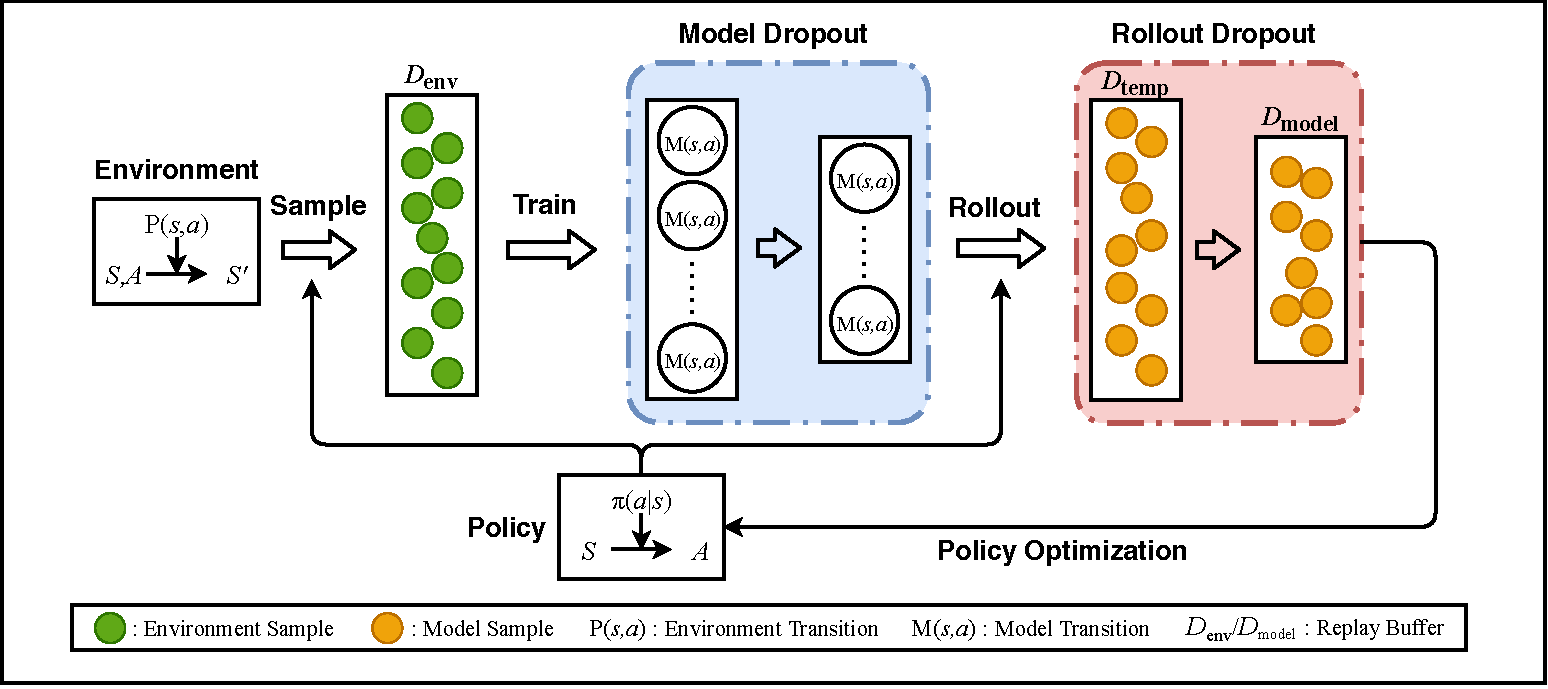
\includegraphics[width=\textwidth]{figures/mbdp.pdf}
\caption{算法整体框架结构。}
\label{fig:algo-structure}
\end{figure}

由于在强化学习中模拟误差越小,算法的收敛性能则越好,观察公式(\ref{eq:MBDP-bound})中的误差上界$D_{\alpha,\beta}(\mathcal{M})$可知,强化学习的算法性能与参数$\alpha$成反比,与参数$\beta$成正比,又根据\ref{sec:model-method}节和\ref{sec:rollout-method}节的介绍可知,策略的鲁棒性显然与参数$\alpha$成正比,与参数$\beta$成反比,恰好与前面的作用效果相反。

因此,本论文可以动态性地调整参数$\alpha,\beta$来取得算法性能和最终策略鲁棒性之间的平衡,从而得到不同属性的强化学习决策策略:

\begin{itemize}
    \item \textbf{平衡的决策策略}:将参数$\alpha$和$\beta$调整为适中大小的概率值,适用于一般的普通环境;
    \item \textbf{收益性能较高的决策策略}:将参数$\alpha$调整为较小的概率值,$\beta$调整为较大的概率值,适用于相对稳定的环境;
    \item \textbf{鲁棒性较好的决策策略}:将参数$\alpha$调整为较大的概率值,$\beta$调整为较小的概率值,适用于干扰较大的环境。
\end{itemize}

基于\ref{sec:model-method}节和\ref{sec:rollout-method}节的提出的改进方案思路,将其整合进传统的基于模型的强化学习算法框架,得到改进的算法,算法整体框架如图\ref{fig:algo-structure}所示。

首先通过与环境交互产生样本,用于训练概率模型并集成模拟,两个筛选模块作为主要改进加入到模拟数据生成的环节中,最终提供给策略优化公式对策略$\pi(a|s)$进行优化,并进行下一轮迭代。
